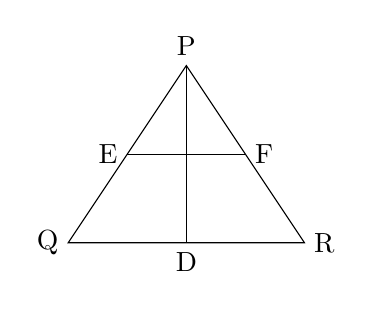
\begin{tikzpicture}[scale=1.5]
    \coordinate (P) at (1,1.5);
    \coordinate (Q) at (0,0);
    \coordinate (R) at (2,0);
    \coordinate (E) at (0.5,0.75);
    \coordinate (F) at (1.5,0.75);
    \coordinate (D) at (1,0);

    \draw (P) -- (Q) -- (R) -- cycle;
    \draw (E) -- (F);
    \draw (P) -- (D);

    \node[above] at (P) {P};
    \node[left] at (Q) {Q};
    \node[right] at (R) {R};
    \node[left] at (E) {E};
    \node[right] at (F) {F};
    \node[below] at (D) {D};
\end{tikzpicture}